%%%%%%%%%%%%%%%%%%%%%%%%%%%%%%%%%%%%%%%%%%%%%%%%%%%%%%%%%%%%%%%%%%%%%%%%%%%%%%%%
%2345678901234567890123456789012345678901234567890123456789012345678901234567890
%        1         2         3         4         5         6         7         8

%\documentclass[letterpaper, 10 pt, conference]{orbieeeconfpre}  % Comment this line out if you need a4paper

\documentclass[a4paper, 10pt, journal]{wissarbIEEE}      % Use this line for a4 paper
%\conference{IEEE Conference for Awesome ORB Research}

\bibliographystyle{orbref-num}

\overrideIEEEmargins                                      % Needed to meet printer requirements.

% See the \addtolength command later in the file to balance the column lengths
% on the last page of the document

\usepackage{hyperref}
\usepackage{graphicx}
\usepackage{tabularx}
\usepackage{booktabs}
\usepackage{lipsum}

\title{\LARGE \bf Scientific Work Short Paper \\Feasibility Study - SmartWarehouse}

\author{Felix Hausberger and Robin Kuck}

\begin{document}
	
	% tense

\maketitle

%%%%%%%%%%%%%%%%%%%%%%%%%%%%%%%%%%%%%%%%%%%%%%%%%%%%%%%%%%%%%%%%%%%%%%%%%%%%%%%%
\begin{abstract}

In this short paper the object detectors \textit{You Only Look Once} and \textit{Single Shot MultiBox Detector} are compared for precision, reactivity, training and inference behaviour and examined for their potential for industrial use. The background scenario of the Smart Warehouse offers live video data of a drone with goods in a warehouse, which are to be classffied and localized in real time. In the future, this should make it possible to carry out inventories and inventory analyses of a warehouse in a time- and cost-efficient manner conserving resources.

The goal of this feasibility study is to find out whether the Smart Warehouse scenario is technically feasible. In addition, the focus is also on the object detectors themselves, their differences in architecture, behavior and how well they are generally suitable for industrial application scenarios.

\end{abstract}

%%%%%%%%%%%%%%%%%%%%%%%%%%%%%%%%%%%%%%%%%%%%%%%%%%%%%%%%%%%%%%%%%%%%%%%%%%%%%%%%
\section{Introduction}

Object detection represents a major field of study in industrial fields like autonomous driving, industrial processing or even government monitoring. Especially in times of the industrial change towards Industry 4.0 such object detectors represent an optimization potential not to be neglected, e.g. in warehousing and logistics. Combined with an autonomous drone, such object detectors could make it possible to conduct inventory checks in a warehouse without human assistance. How different object detectors behave when applied to a real time industry scenario like \textit{SmartWarehouse} should be evaluated in this short paper. As being a feasibility study, the main goal of this work also is to discuss the feasibility of the \textit{SmartWarehouse} idea based on the performance of the two selected object detectors \textit{You Only Look Once} (YOLO) and \textit{Single Shot MultiBox Detector} (SSD) in terms of precision, responsiveness, training and inference behavior. In \autoref{relatedwork} related work to similar industry scenarios should be introduced before explaining the approach and architecture of the \textit{SmartWarehouse} prototype in \autoref{architecture}. In \autoref{evaluation} the results of the feasibility study will be presented and evaluated before the interpretability of the results is discussed in \autoref{results}. \autoref{conclusion} gives a quick coonclusion about the main achievements of this short paper.

\section{Related Work} \label{relatedwork}

The idea of automized inventory checks with drones is not new. \cite{doks.innovationGmbH.2020} uses a similar approach, but uses normal RFID technology or simple barcodes to identify a product. Using this approach only a small number of instances at a time can be identified, while using object detection algorithms enable many-numbered and faster processing. 

The paper \cite{WeiLiuDragomirAnguelovDumitruErhanChristianSzegedyScottReedChengYangFuAlexander.2016} introduces the \textit{Single Shot MultiBox Detector} (SSD), an object detector reaching up to 76.9\% mean average precision (mAP) while still keeping real time detection characteristics compared to its preceeding competitors like regional convolutional neural networks (R-CNNs). It uses a single neural network to detect objects and creates a set of default bounding boxes over different aspect ratios and scales for each feature map location instead of using an additional bounding box proposal step. 

The \textit{You only Look Once} (YOLO) algorithm was introduced in \cite{JosephRedmonSantoshDivvalaRossGirshickAliFarhadi.2016} and as well uses a single neural network to predict bounding boxes and class probabilities. Incremental improvements led to version three of YOLO, which is equally accurate as SSD, but three times faster \cite{JosephRedmon.2018}. 

\section{Architecture of the SmartWarehouse scenario} \label{architecture}

\subsection{Defining the scenario}

Two goals were defined for the feasibility study of \textit{SmartWarehouse}. First it is to be evaluated, how well existing object detectors perform in industry scenarios taking the example of \textit{SmartWarehouse} and the two object detectors YOLO and SSD. Second, one should deal with the feasibility of the implementation of this \textit{SmartWarehouse} scenario, which comprises the execution of an inventory for department stores with a drone. 

\subsection{Dataset}

The \textit{SmartWarehouse} is based on a large department store, where products are not packed in
are not packed in cartons, but are arranged as a whole on shelves. In the construction of the training data set, however, the feasibility study does not aim to represent such a store completely in the data set, but rather to select a dataset that is as extensive as possible in order to prove the general feasibility of the \textit{SmartWarehouse} scenario. In the context, the focus was therefore on beverage bottles of a department store. Nine categories were defined: \textit{Saskia Water Small}, \textit{Saskia Water Large}, \textit{Pepsi Cola Small}, \textit{Pepsi Cola Large}, \textit{ISO}, \textit{ACE}, \textit{Stenger Blackcurrant Spritzer}, \textit{Stenger Apple Spritzer}, and \textit{Vitamalz Malt Beer}. All classes are distributed equally in the data set. The data set itself is 1.45 GB big and consists of 1088 manually annotated images of resolution 2112x4608 and 24 bit color depth. The annotations are given in \textit{PascalVOC} and \textit{YOLO} format. 75\% of the images include a single instances of a beverage bottle to better train the patterns of the different classes. Furthermore, 13\% of the images contain occlusions of objects to be detected, detection situations from extreme viewing positions are represented to 4\%, and difficult illumination and lighting conditions are included to 8\%. Only a few examples (2\%) are related to different distances during detection. Care was also taken to continuously vary the backgrounds of the objects being detected. With the enrichment of the data set with representations of such difficult recording circumstances, it is hoped to increase the generalization capability of Deep Learning models based on them. Finally, to simulate the department store where several objects are to be detected at once, in 12.5\% of all images the objects are arranged on shelves, one behind the other or in beverage crates. From the total dataset of 1088 images, 90 images were extracted for later validation. The remaining 998 consist of 200 images of test data and 798 images for training. In 90\% of all images, only objects of one class are shown, since commodity inventories are likewise mostly grouped by commodity. The dataset was published on Kaggle\footnote{see \url{https://www.kaggle.com/fidsusj/smartwarehousessd} and \url{https://www.kaggle.com/fidsusj/smartwarehouseyolo}} for both PascalVOC format and YOLO format.

\subsection{Introduction of evaluation criteria}

To better compare object detectors with each other the following evaluation criteria have been defined:

\begin{itemize}
	\item Precision: The precision of an object detector measured in mAP
	\item Reactivity: The inference rate with the model measured in \textit{Frames Per Second} (FPS)
	\item Training behavior: The speed of the gradient curve until convergence measured in training epochs
	\item Inference behavior: The inference behavior under special lighting conditions, extreme viewing positions, occultation of objects, and the behavior with double detected objects measured with good, medium, poor. 
\end{itemize}

\subsection{Selection of object detectors}

For the smart warehouse scenario, a choice should be made between the four detectors Faster R-CNN, Mask R-CNN, SSD and YOLO. 

\begin{figure}[h]
	\centering
	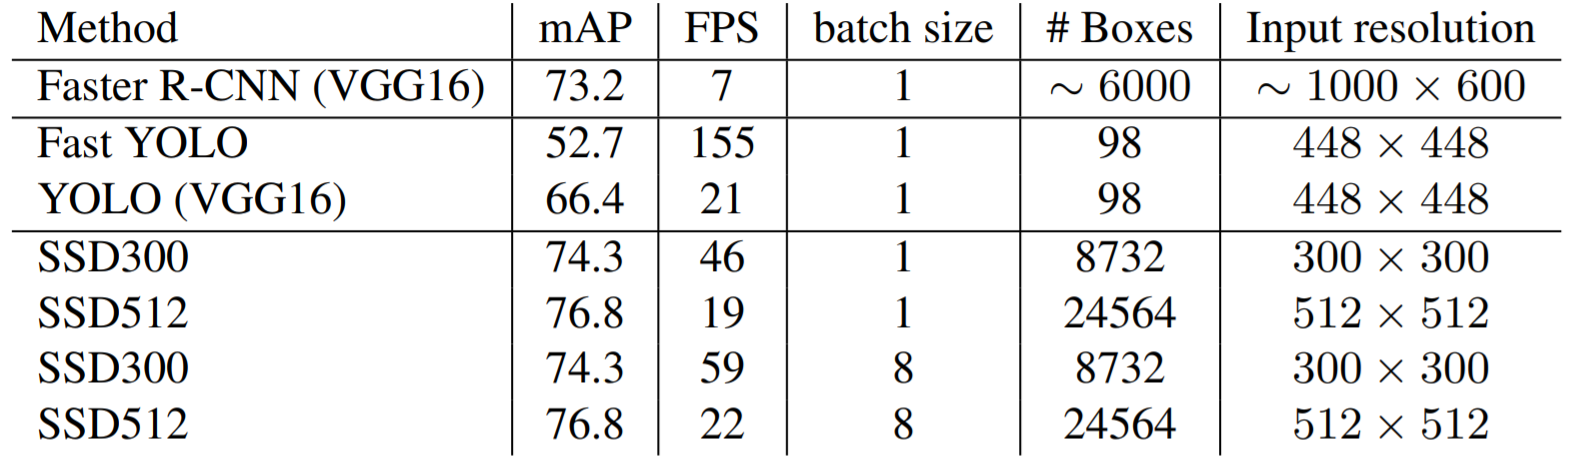
\includegraphics[width=0.5\textwidth]{fig/ssd_results.png}
	\caption{Comparison of SSD on PascalVOC 2007 \cite{WeiLiuDragomirAnguelovDumitruErhanChristianSzegedyScottReedChengYangFuAlexander.2016}}
	\label{ssd_results}
\end{figure}

According to the reference results in \autoref{ssd_results}, it is clear that the SSD performs best in terms of mAP with 74.3\% and 76.8\%, respectively. Faster-RCNN can keep up with 73.2\% in terms of mAP,
but with only 7 FPS it is not designed for fast inference. YOLO scores worse than the SSD in both categories, it essentially achieves an mAP of 66.4\% and a frame rate of 21 FPS. The SSD thus manages to maintain a good balance between precision and responsiveness. Comparing Mask-RCNN from the original paper in \cite{KaimingHeGeorgiaGkioxariPiotrDollarRossGirshick.2018} with Faster-RCNN (RoI-Align) results in a mAP difference of 38.2\% to 37.3\%. Only 5 FPS could be reached. 

To find two suitable object detectors to evaluate, the effort setup the implementations and to adapt them to be trained with a custom data set was also taken into account. Whereas the SSD and YOLO implementations were easy to handle regarding these two tasks, implementations of ferster-RCNN or Mask-RCNN were either not supported on the operating system of choice or already depricated and no longer supported. 

Due to these circumstances and the poorer performance in time-critical model inference, YOLO and SSD were selected as the two detectors to evaluate the capability of object detectors for industrial use using the smart warehouse scenario as an example. The official implementation of YOLOv3 in the \textit{Darknet} framework and a custom implementation of SSD300 in the \textit{PyTorch} framework is used.

\subsection{Training infrastructure}

When selecting the training infrastructure, cloud PaaS offerings were first considered. Important factors in the selection process were the lowest possible operating costs, a diverse range of hardware accelerators, and simple setup of the training infrastructure. In particular, the test versions of the respective offerings should be taken advantage of in order to achieve low operating costs.

\textit{Amazon SageMaker} did not offer cloud GPUs as a hardware accelerators at all in its free trial version, which is why is was elimitated from the selection. Similarly, the not enough quota was available for the \textit{Deep Learning VM} from the  \textit{Google Cloud Platform}. However, since Microsoft Azure's offering was only described very superficially, the decision was ultimately also made against Microsoft Azure.

The exlusion of the three hyperscalar offerings led to \textit{FloydHub} as another deep learning platform. Here hardware accelerated GPUs were freely accessible from the very beginning until a certain time throshold was reached based on the GPU model. During the training with the NVIDIA Tesla K80, however, it was noticeable that the choice of this GPU did not bring any major performance improvements compared to local training.It is noticeable that an NVIDIA Tesla K80 can keep up with the existing local graphics cards in the degree of parallelization, but scores far worse in the number of computing operations per second. Compared to an NVIDIA GeForce GTX 1080, the NVIDIA Tesla K80 performs less than half as fast in terms of computing power. For work-related reasons, it should be noted that the two object detectors SSD and YOLO are each trained locally on different hardware, SSD on an NVIDIA GeForce GTX 1080 and YOLO on an NVIDIA GeForce RTX 2060 GPU. Therefore, it was made use of NVIDIAs' \textit{Compute Unified Device Architecture} (CUDA) as a programming model and parallel computing platform to offload computing power to the GPUs. Also the NVIDIA \textit{CUDA Deep Neural Network Library} (cuDNN) was used, which offers hardware-optimized routines for convolution or pooling operations. 

\subsection{Drone selection}

Analyzing the market for programmable drones with a freely available software development kit (SDK) and integrated camera, the supply is very low. The choice restricts to either the \textit{Parot Bebop II} or the \textit{Ryze Tello EDU}. When also taking into account the legal framework, only the \textit{Ryze Tello EDU} was left for legal usage.

\subsection{Inventory software specification}

To process the drone's image data for an inventory, the drone is to be accessed by a client application. The server, acting as a client, is to connect to the drone and sends the flight signals as static flight instructions to the drone. The deep learning model is also to be integrated on the server for inference. The server's task will be to infer the video stream frames received from the drone with the model, count the detected objects for the inventory using a counting algorithm, and then forward the image data with the bounding boxes drawn in via livestream to a web application for visualization. A REST interface should provide information about the inventory data of the warehouse and provide a way to initiate the flight sequence.

\section{Realization}

\textbf{SSD}. The base network of the SSD consists of a VGG16 pre-trained on ImageNet. The remaining convolutional layers are Xavier initialized. SSD was trainied with a batch size of 16, $1.0e^{-3}$ as learning rate and 0.9 as momentum. ReLU was chosen as its activation function and smooth L1 as its loss function. Using the mini-batch learning approach training was done with six-fold cross validation with 22 epochs each.

\textbf{YOLO}. YOLO was trained with a batch size of 64 and 16subdivisions. The learning rate was $1.0e^{-3}$ initially, then decreased to $1.0e^{-4}$ after 80\%, and to $1.0e^{-5}$ after 90\% of the training process, the momentum was also 0.9. 18.000 batches were specified in total for the mini-batch gradient descent training process. LReLU was chosen as the activation function and squared errors as the loss function.

\textbf{Counting algorithm}. After each inference process, the detected objects are saved so that the algorithm can access both the most recently detected objects and the newly detected objects when it is called. For all detected objects in the current run, the algorithm searches all last detected objects to find out if an object was already present in the previous image. Crucial for this is the same label as well as the distance of the bounding boxes of the currently detected object to the object of the previous round. Only if the object was not already present in the previous round according to these criteria, it is counted.

\textbf{Drone connection}. For control and access to the video stream, the Ryze Tello EDU offers its own WiFi network to which the control unit must connect. The communication takes place via the UDP protocol1 and consists of several communication channels. The sending of flight commands and the polling of the video stream is done via a bidirectional socket connection between the client application and the Ryze Tello EDU.

\textbf{Model inference}. Since the H.264 decoder can only run on Python version 2.7 and the PyTorch framework used for the SSD or the Darknet framework for YOLO can only run on Python version 3, it was not possible to allow inference of live video data from the drone. Python version 3 is generally not backward compatible with previous versions, so the H.264 decoder required by the Ryze Tello EDU SDK was not compatible with the existing infrastructure. Because of this, it was decided to simplify the problem by inferring images from a webcam instead of images from the drone.

\section{Results and evaluation} \label{evaluation}

SSD reached an mAP score of 83.1\%, while YOLO scores almost equally high with 80.4\%. To minimize double detected objects the confidence score for SSD was set to 0.7, for YOLO already 0.25 was enough. SDD struggles to detect partly hidden objects. Also detecting objects from extreme view positions was difficult, but can be improved by adding more samples for this case. For those special cases YOLO performs equally bad, for the latter even worse. SSD reliably detects objects until a three meters distance threshold, YOLOs' maximum range is only two meters. Overlit lighting conditions leads to no or wrong object detection using the SSD or YOLO algorithm. However, all detections of both models reacted invariantly to different backgrounds or image resolutions. 

Both SSD and YOLO are capable to run inference in the real time scenario of \textit{SmartWarehouse}, SSD with 30 PFS and YOLO with 28 FPS. 

SSD took 16.5 hours to train, whereas YOLO took 8 hours. Nevertheless, as both algorithms were trained on different hardware, use different frameworks and use different batch sizes, the results cannot be really compared. 

\section{Discussion} \label{results}

\section{Conclusion} \label{conclusion}

\bibliography{mybibfile}

\end{document}
